\documentclass{beamer}
\usepackage{amsmath,amsthm,bm,bbm}
\usepackage[justification=centering]{subcaption}
\usepackage[justification=centering]{caption}
\usepackage{graphicx}
\usepackage{csquotes}
\usepackage[style=apa, backend=biber]{biblatex}
\addbibresource{lit.bib}

\logo{
\includegraphics[scale=0.1]{ETS-Logo-navy-gold.png}}

\setbeamertemplate{footline}[frame number]
\setbeamertemplate{headline}{}

\title{Conditionally Unbiased Best Linear Predictors for Score Augmentation}
\author{Xiang Liu, Matthew S. Johnson, Sandip Sinharay}
\institute{Educational Testing Service}
\date{\today}

%% new commands %%
\newcommand{\mbf}[1]{\bm{#1}}
\newcommand{\bc}{\mbf{c}}
\newcommand{\bX}{\mbf{X}}
\newcommand{\bY}{\mbf{Y}}
\newcommand{\bT}{\mbf{T}}
\newcommand{\C}{\mathcal{C}}
\newcommand{\bbeta}{\mbf{\beta}}
\newcommand{\bmu}{\mbf{\mu}}
\newcommand{\beps}{\mbf{\varepsilon}}
\newcommand{\btau}{\mbf{\tau}}
\newcommand{\bgamma}{\mbf{\gamma}}
\newcommand{\blambda}{\mbf{\lambda}}
\newcommand{\bW}{\mbf{W}}
\newcommand{\bsigma}{\mbf{\Sigma}}
\newcommand{\E}{\mathbb{E}}
\newcommand\independent{\protect\mathpalette{\protect\independenT}{\perp}}
\def\independenT#1#2{\mathrel{\rlap{$#1#2$}\mkern2mu{#1#2}}}
\DeclareMathOperator{\MSE}{MSE}
\DeclareMathOperator{\Cov}{Cov}
\DeclareMathOperator{\Var}{Var}
%%%%%%%%%%% 

\begin{document}
	\frame{\titlepage}

	\begin{frame}[t]\frametitle{Background}
	\begin{itemize}
		\item Assessments transition from being paper-pencil based to digital.
		\item The Big Data movement.
		\item Additional information about the construct of interest comes from
		different sources.
		\item In writing assessments - scores from multiple raters, product features
		(e.g. NLP related ones from the e-rater\textsuperscript{\textregistered}),
		and process features from keystroke logs, etc.
		\item The goal is to make inferences about the writing ability combining all
		these information.
		\item Augmenting the rater scores with additional information.
		\item The same can be generalized to other assessments - math, reading,
		speaking, etc.
	\end{itemize}
	\end{frame}

	\begin{frame}[t]\frametitle{Motivation}
	\begin{itemize}
		\item The best linear predictors (BLP) has been proposed to combine sources
		of information to predict some latent true score (e.g. augmenting writing
		proficiency estimate with scores from other sections; 
		\cite{Haberman2015,Yao2019}).
		\item "Predicting" random effects vs. "estimating" fixed effects.
		\item The BLP minimizes the MSE of prediction; However, its exhibits
		shrinkage towards the population mean \parencite{Robinson1991}.
		\item The BLP may biased conditional on the true score level (i.e. for 
		individual students). It could lead to fairness concerns (e.g. favoring
		certain groups over others). 
		\item We need an approach that is conditionally unbiased (or unbiased at
		individual level).
	\end{itemize}
	\end{frame}

	\begin{frame}[t]\frametitle{The model}
	\begin{itemize}
		\item $\bY = (Y_1, Y_2, \dots, Y_J)^\top$ is the vector of variables
		measured with error (i.e. manifest variables of some latent variable of
		interest. e.g.essay scores from raters).
  	\item $\bX = (X_1, X_2, \dots, X_K)^\top$ is the vector of variables
  	measured without error (i.e. covariates that may correlate with the latent
  	trait, e.g. typing speed).
  	\item \begin{equation}
				    \mbf{W} = \left (
				      \begin{array}{c} \bY \\  \bX \end{array} \right ) =
				    \mbf{\alpha} + \mbf{\lambda} S + \mbf{\varepsilon}_w.
				  \end{equation},
				  where $S$ is the latent variable and $\mbf{\varepsilon}_w$ denotes the
				  residuals.
		\item For mathematical convenience, we center $\bW$,
		\begin{equation}
		\label{eq:linear_model}
    	\bW = \blambda S + \mbf{\varepsilon}_w,
  	\end{equation}
  	$E(S) = 0$, $E(\beps_w) = \mbf{0}$, and
  	\begin{equation*}
	    \Cov\left(\begin{array}{c} S \\ \beps_w \end{array}\right) = \begin{bmatrix}
	      \sigma_S^2 & 0 \\
	      0 & \bsigma_{\beps_w}
	    \end{bmatrix}.
	  \end{equation*}
  \end{itemize}
	\end{frame}

	\begin{frame}[t]\frametitle{Example models}
		\begin{figure}
	    \begin{subfigure}{0.45\textwidth}
	      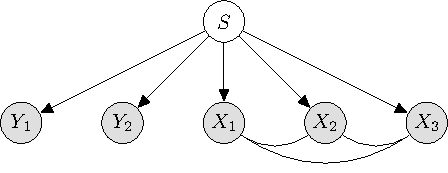
\includegraphics[width=\textwidth]{Fig/model_1.pdf}
	      \caption{Correlated residuals of $X$}
	    \end{subfigure}\hfill
	    \begin{subfigure}{0.45\textwidth}
	      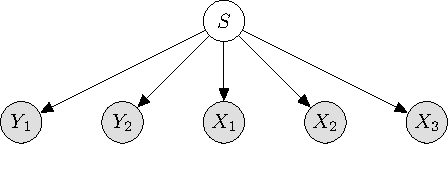
\includegraphics[width=\textwidth]{Fig/model_2.pdf}
	      \caption{Uncorrelated residuals of $X$}
	    \end{subfigure}
	    \caption{Graphical representation of some example models}
	    \label{fig:PGM_example}
  	\end{figure}
  \begin{itemize}
  	\item The model is flexible. Depending on the structure of $\bsigma_
  	{\beps_w}$, it can describe a broad class of models.
  \end{itemize}
	\end{frame}

	\begin{frame}[t]\frametitle{BLP}
	\begin{itemize}
		\item BLP, $\hat{S} = \bgamma_1^\top \bW$, minimizes the mean squared error
		for prediction\footnote{assumes $E[\beps_w|S] = 0$}, 
		\begin{equation}
			\MSE = E[(S - \bgamma_1^\top \bW)^2] = \sigma_S^2 + \bgamma_1^\top
			\bsigma_{\bW} \bgamma_1 - 2\bgamma_1^\top \blambda \sigma_S^2 
    \end{equation}
    \item BLP is obtained by solving
    \begin{align}
	    \nabla \MSE &= \nabla(\bgamma_1^\top \bsigma_{\bW} \bgamma_1)  - \nabla
	    (2\bgamma_1^\top \blambda \sigma_S^2) \\
	    &= 2\Sigma_{\bW} \bgamma_1 - 2 \blambda \sigma_S^2 = 0,
	  \end{align}
	 	\item The BLP coefficients are $\bgamma_1 = \Sigma_{\bW}^{-1} \blambda
	 	\sigma_S^2$. By the decomposition $\Sigma_{\bW} =
	 	\sigma_S^2\blambda\blambda^\top + \bsigma_{\mbf{\varepsilon}_w}$ and the
	 	Woodbury matrix identity, the coefficients can be alternatively expressed
	 	as 
	 	\begin{equation}
	    \bgamma_1 = \frac{\Sigma_{\mbf{\varepsilon}_w}^{-1}\blambda}{1/\sigma_S^2 +
	    \blambda^\top\Sigma_{\mbf{\varepsilon}_w}^{-1}\blambda}.
	  \end{equation}
	\end{itemize}
	\end{frame}

	\begin{frame}[t]\frametitle{Bias}
		\begin{itemize}
			\item \textbf{Averaged over the population}, the BLP is unbiased, i.e.
			  \begin{align}
			    Bias(\hat{S}) &= E[\hat{S} - S] \nonumber\\
			    &= E[(\sigma_S^2\blambda^\top \Sigma_{\bW}^{-1})\bW - S]\\
			    &= \sigma_S^2\blambda^\top \Sigma_{\bW}^{-1} E[W] - E[S] = 0.
			  \end{align}
			\item The BLP can be biased \textbf{for individuals} (or conditional $S$),
			\begin{align}
		    E[\hat{S} - S|S] &= E[\sigma_S^2\blambda^\top\Sigma_{\bW}^{-1}\bW|S] - S
		    \nonumber\\
		    &= E[\sigma_S^2\blambda^\top\Sigma_{\bW}^{-1}(\blambda S + 
		    \mbf{\varepsilon}_w)|S] - S \nonumber\\
		    &= S(\sigma_S^2\blambda^\top\Sigma_{\bW}^{-1}\blambda - 1). 
		    \label{eq:conditional_bias}
		  \end{align}
		  \item The conditional bias depends on $S$ and the ratio
		  $\sigma_S^2\blambda^\top\Sigma_{\bW}^\top\blambda$. 
		\end{itemize}
	\end{frame}

	\begin{frame}[t]\frametitle{Figure: Conditional bias under different
	covariance ratios}
		\begin{figure}[t]
	  \centering
	    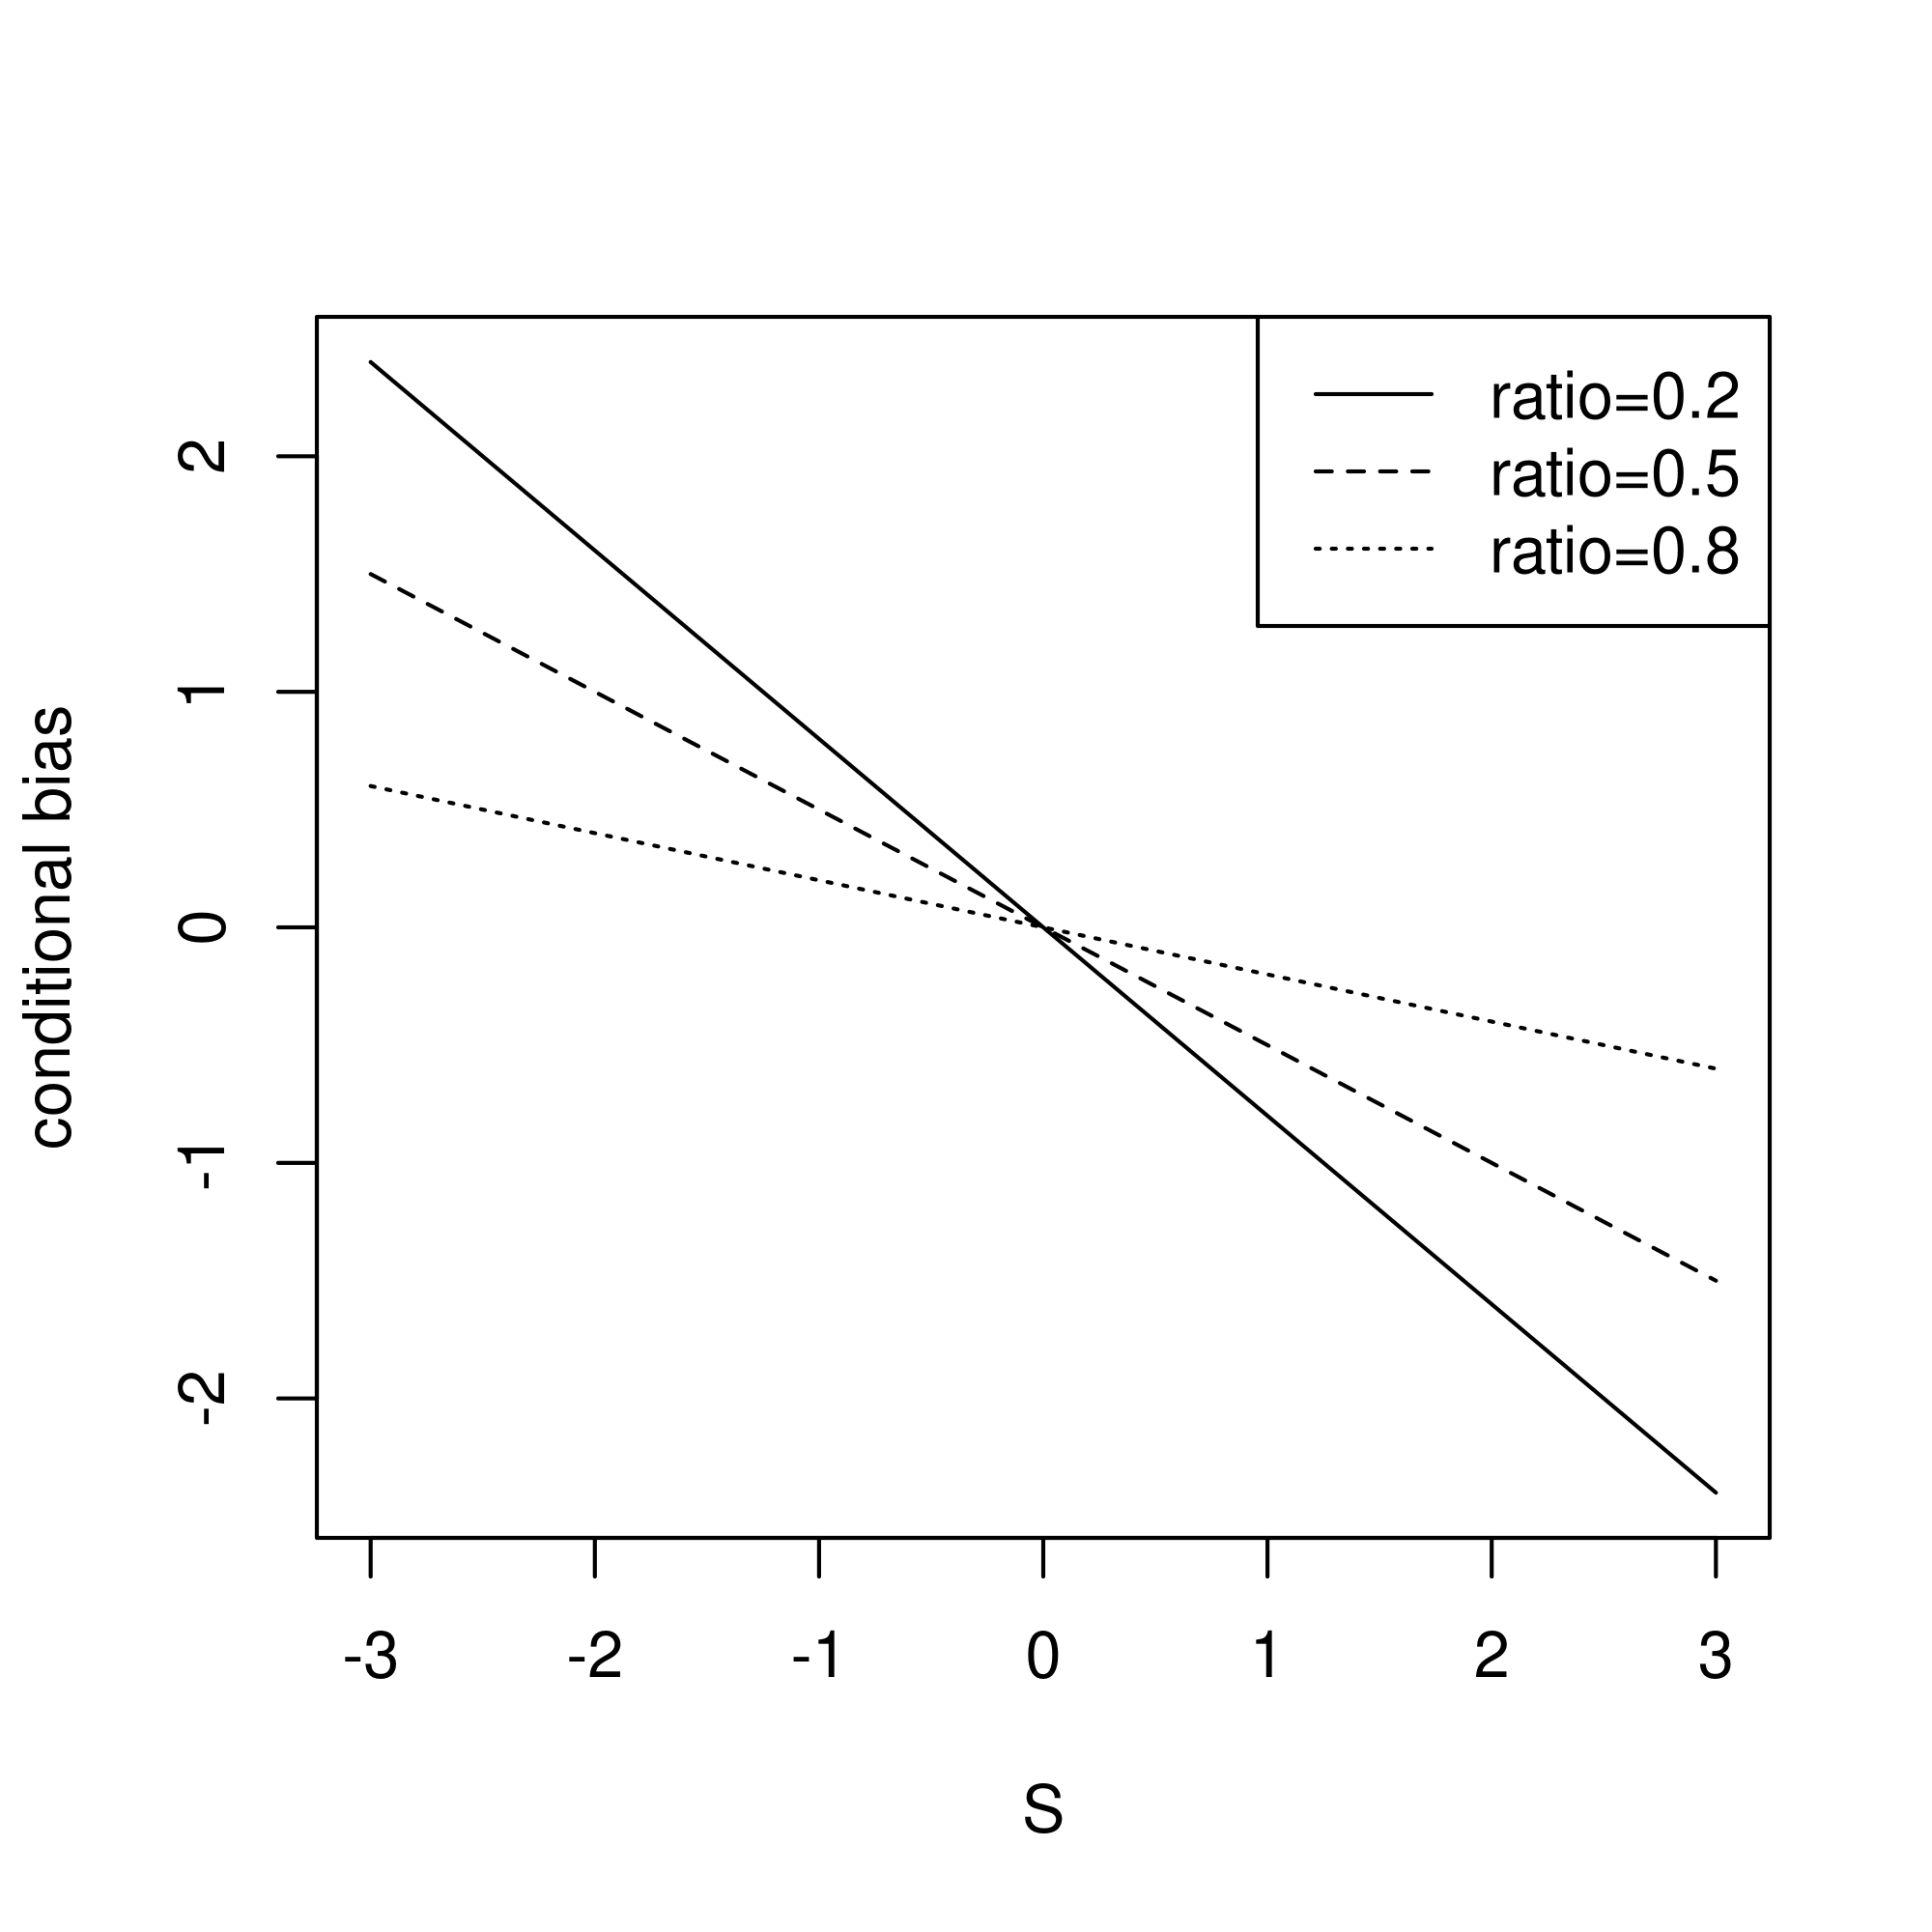
\includegraphics[scale = 0.6]{Fig/conditional_bias.png}
	  \end{figure}
	\end{frame}

	\begin{frame}[t]\frametitle{CUBLP}
		\begin{itemize}
			\item The CUBLP, $\hat{S} = \bgamma_1^\top \bW$, minimizes the MSE $E[(S -
			\bgamma_1^\top \bW )^2]$, subject to
			\begin{equation}
				E[\bgamma_1^\top\bW|S] = \bgamma_1^\top E[\bW|S] = \bgamma_1^\top 
				(\blambda S + E[\mbf{\varepsilon}_w|S]) = S.
			\end{equation}
			\item With the assumption $E(\mbf{\varepsilon}_w|S) = 0$, the constraint
			reduces to $\bgamma_1^\top \blambda = 1$.
			\item This constrained optimization problem can be solved by the method of
			Lagrange multipliers. The Lagrange function is $\mathcal{L} (\blambda_1,
			\delta) = -E[(S-\bgamma_1^\top \bW)^2] - \delta(\bgamma_1^\top \blambda -
			1)$.
			\item The CUBLP coefficients are obtained by solving $\nabla_{\blambda_1,
			\delta} \mathcal{L}(\blambda_1^\top, \delta) = \mbf{0}$.
			\item $\blambda_1 = \frac{\bsigma_{\bW}^{-1}\blambda}{\blambda^\top
			\bsigma_{\bW}^{-1}\blambda}$ or alternatively $\blambda_1 = \frac{\bsigma_
			{\mbf{\varepsilon}_w}^\top \blambda}{\blambda^\top \bsigma_{\mbf{\varepsilon}_w}^\top
			\blambda}$.
		\end{itemize}
	\end{frame}

	\begin{frame}[t]\frametitle{Figure: Comparison of BLP and CUBLP}
	\centering
		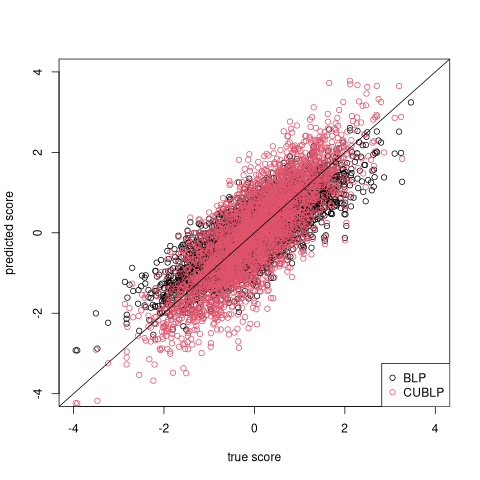
\includegraphics[scale = 0.4]{Fig/prediction.png}
	\end{frame}

	\begin{frame}[t]\frametitle{Parameter estimation}
	\begin{itemize}
		\item BLP and CUBLP coefficients are expressed as functions of the population
		parameters $\blambda$, and $\Sigma_{\bW}$ (or $\mbf{\Sigma}_{\beps_w}$).
		They need to be estimated.
		\item Let $\blambda = \left (\blambda_{\bY}^\top, \blambda_{\bX}^\top
		\right)^\top$ In some applications, it may be desirable or necessary to
		assume $\lambda_{Y_j} = \lambda_{Y}$. We have the covariance decomposition
		\begin{equation}
	  	\mbf{\Sigma}_{\bW} = \blambda \blambda^\top + \mbf{\Sigma}_{\beps},
	  \end{equation},
	  and \begin{equation}
    			\mbf{\Sigma}_{\bY} = \blambda_{\bY} \blambda_{\bY}^\top + \mbf{\Psi}_
    			{\bY},
  			\end{equation}
  	where $\mbf{\Psi}_{\bY}$ is a diagonal matrix.
  	\item A least square (LS) estimator is obtained by minimizing $L(\blambda) =
  	\sum_{k \neq k'} (\lambda_{Y}^2 - r_{Y_k Y_{k'}})^2 + \sum_k \sum_j 
  	(\lambda_Y \lambda_{X_j} - r_{Y_k X_j})^2$
	\end{itemize}
	\end{frame}

	\begin{frame}[t]\frametitle{The LS estimator}
		\begin{itemize}
			\item For equal discrimination cases,
			\begin{equation}
		    \hat{\lambda_Y} = \sqrt{\frac{\sum_{k \neq k'} r_{Y_k Y_{k'}}}{K(K-1)}},
		    \hat{\lambda_{X_j}} = \frac{\sum_k r_{Y_k X_j}}{K\hat{\lambda_Y}}.
		  \end{equation}
		  \item For unequal discrimination cases, iterate through
		  \begin{equation}
		    \hat{\lambda_{Y_k}} = \frac{\sum_{k' \neq k} \lambda_{Y_{k'}} r_{Y_{k}Y_
		    {k'}} + \sum_j \lambda_{X_j} r_{Y_k, X_j}}{\sum_{k' \neq k} \lambda_{Y_
		    {k'}}^2 + \sum_j \lambda_{X_j}^2},
		  \end{equation}
		  and
		  \begin{equation}
		    \hat{\lambda_{X_j}} = \frac{\sum_k \lambda_{Y_k} r_{Y_k X_j}}{\sum_k
		    \lambda_{Y_k}^2}
		  \end{equation}
		 	\item $\bsigma_{\bW}$ can be estimated by the sample covariance matrix or its
		 	ML estimate if distribution assumption is assumed.
		\end{itemize}
	\end{frame}

	\begin{frame}[t]\frametitle{Figure: Behaviors of the LS estimator}
		\begin{figure}[t]
	    \centering
	    \begin{subfigure}[b]{0.45\textwidth}
	      \centering
	      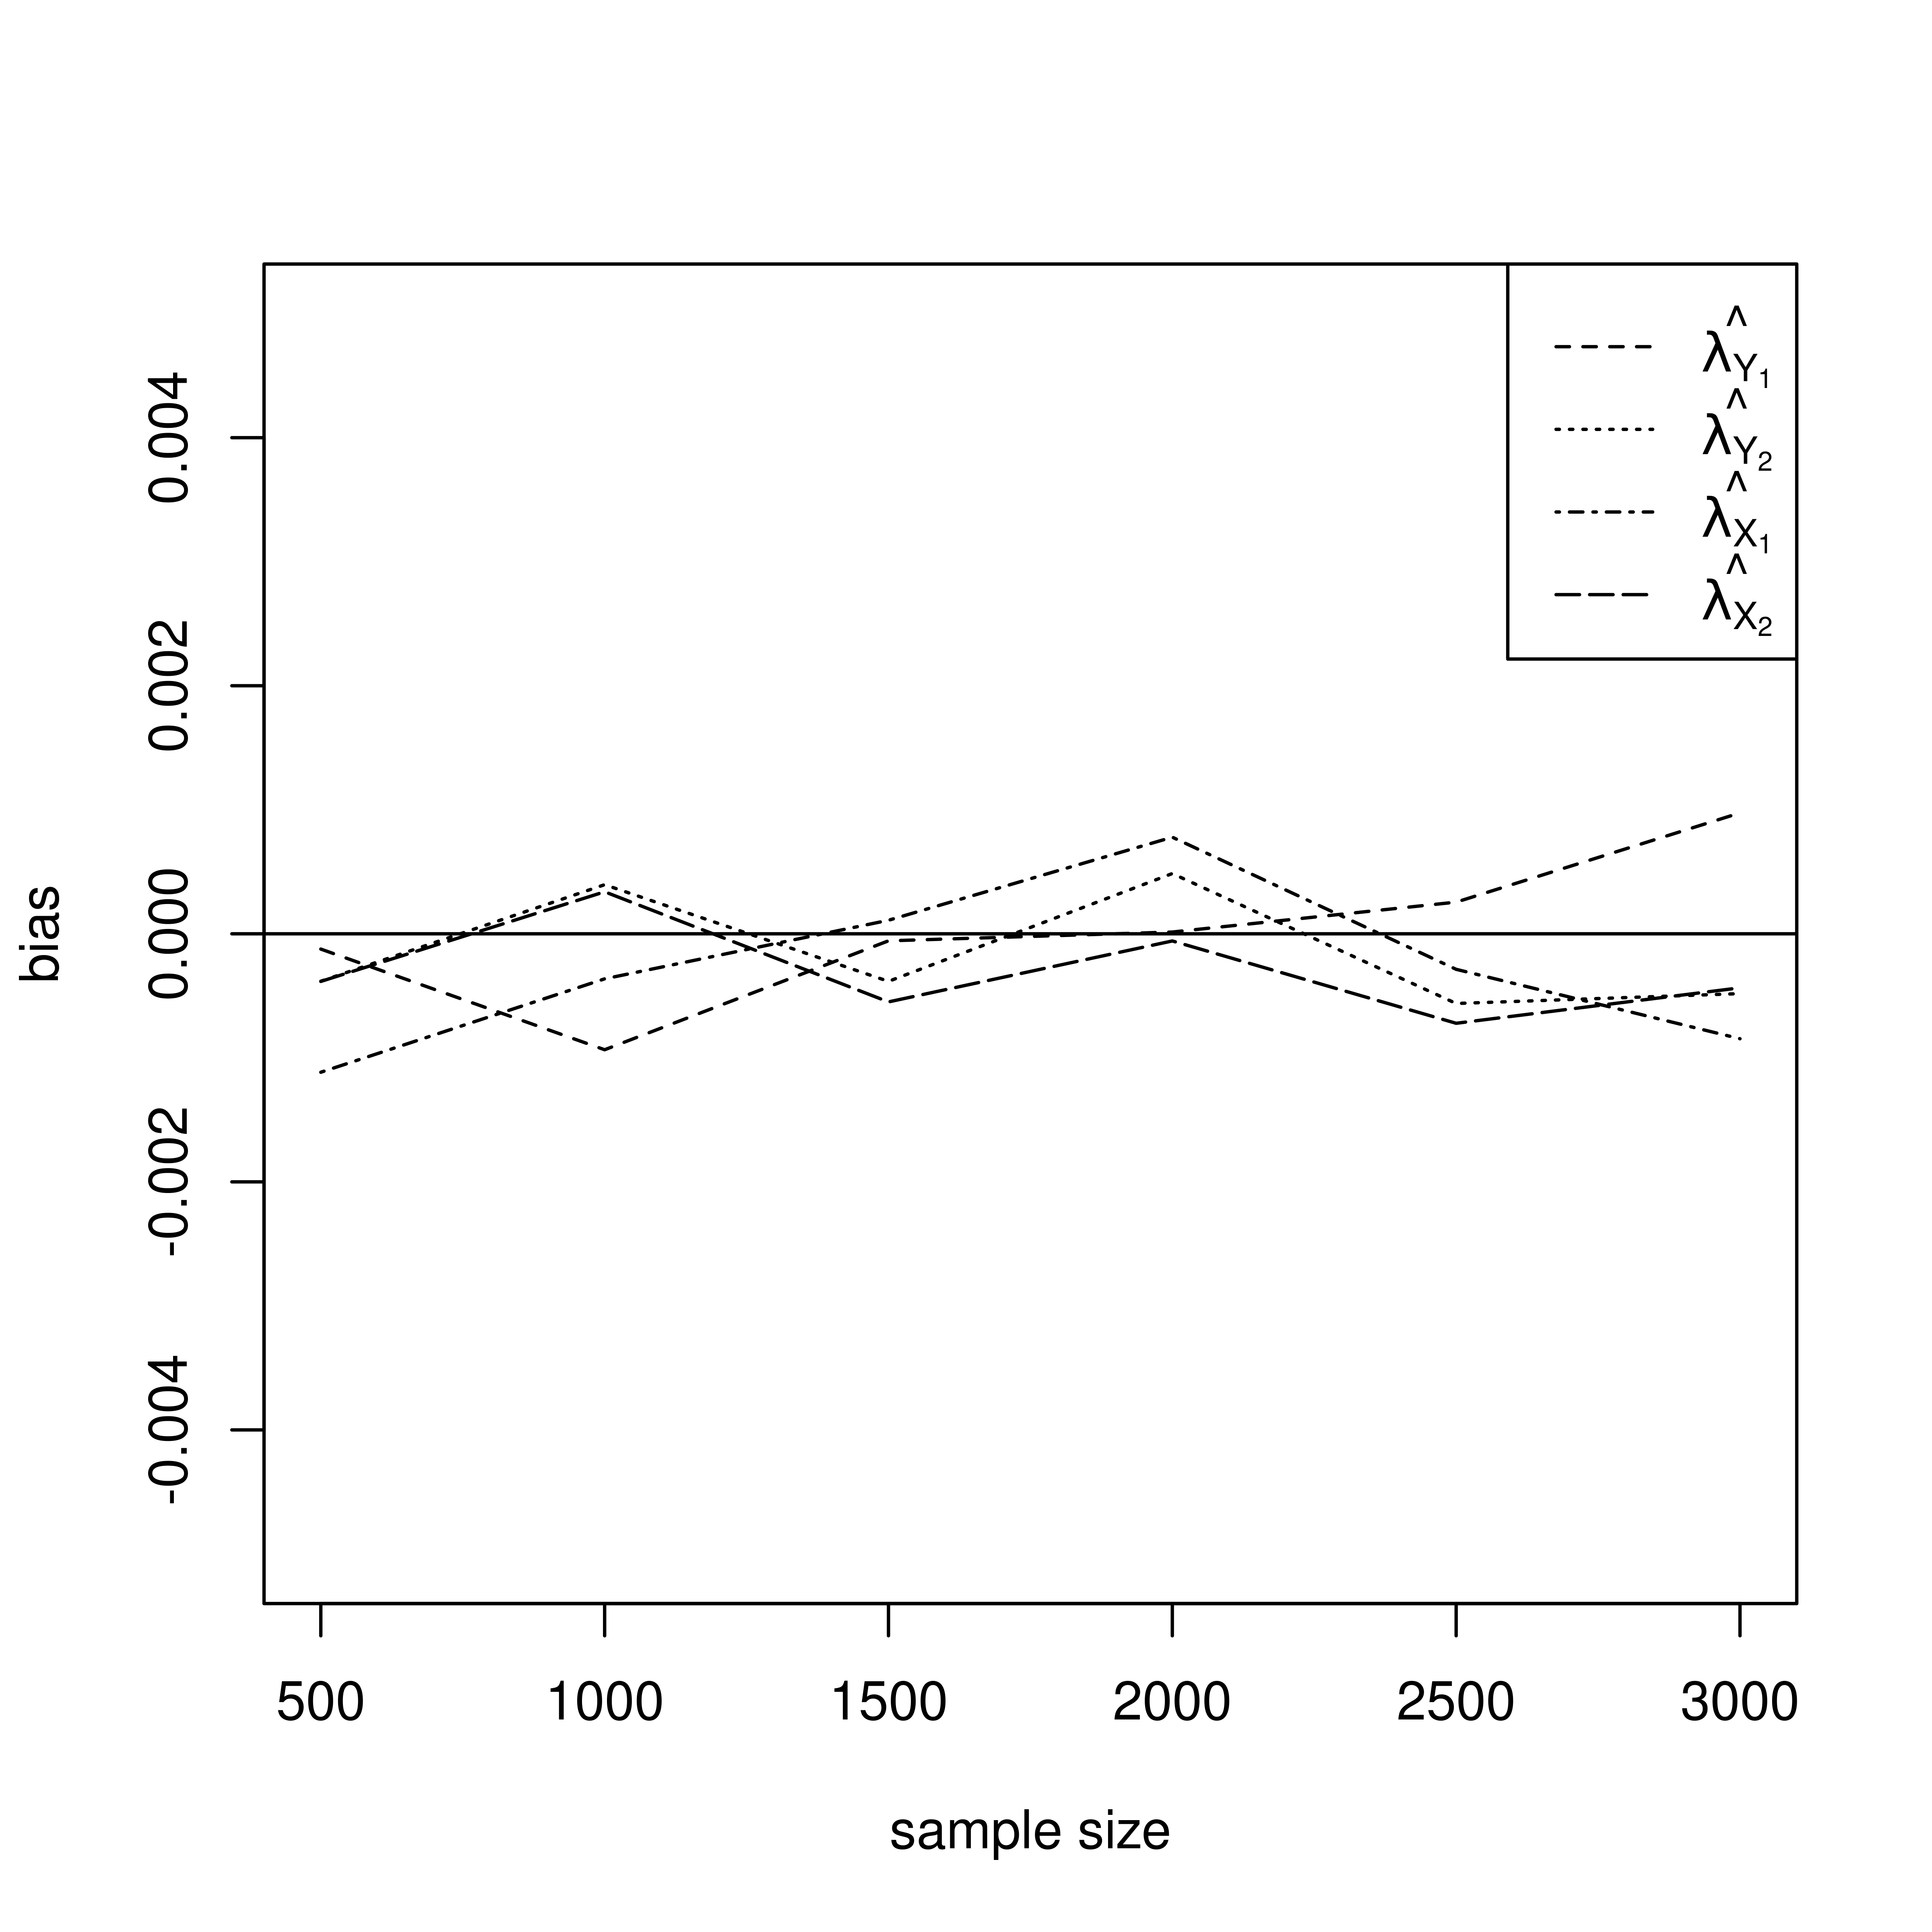
\includegraphics[width=\textwidth]{Fig/bias_uneq_discrim_high.png}
	      \caption{Bias}
	    \end{subfigure}
	    \begin{subfigure}[b]{0.45\textwidth}
	      \centering
	      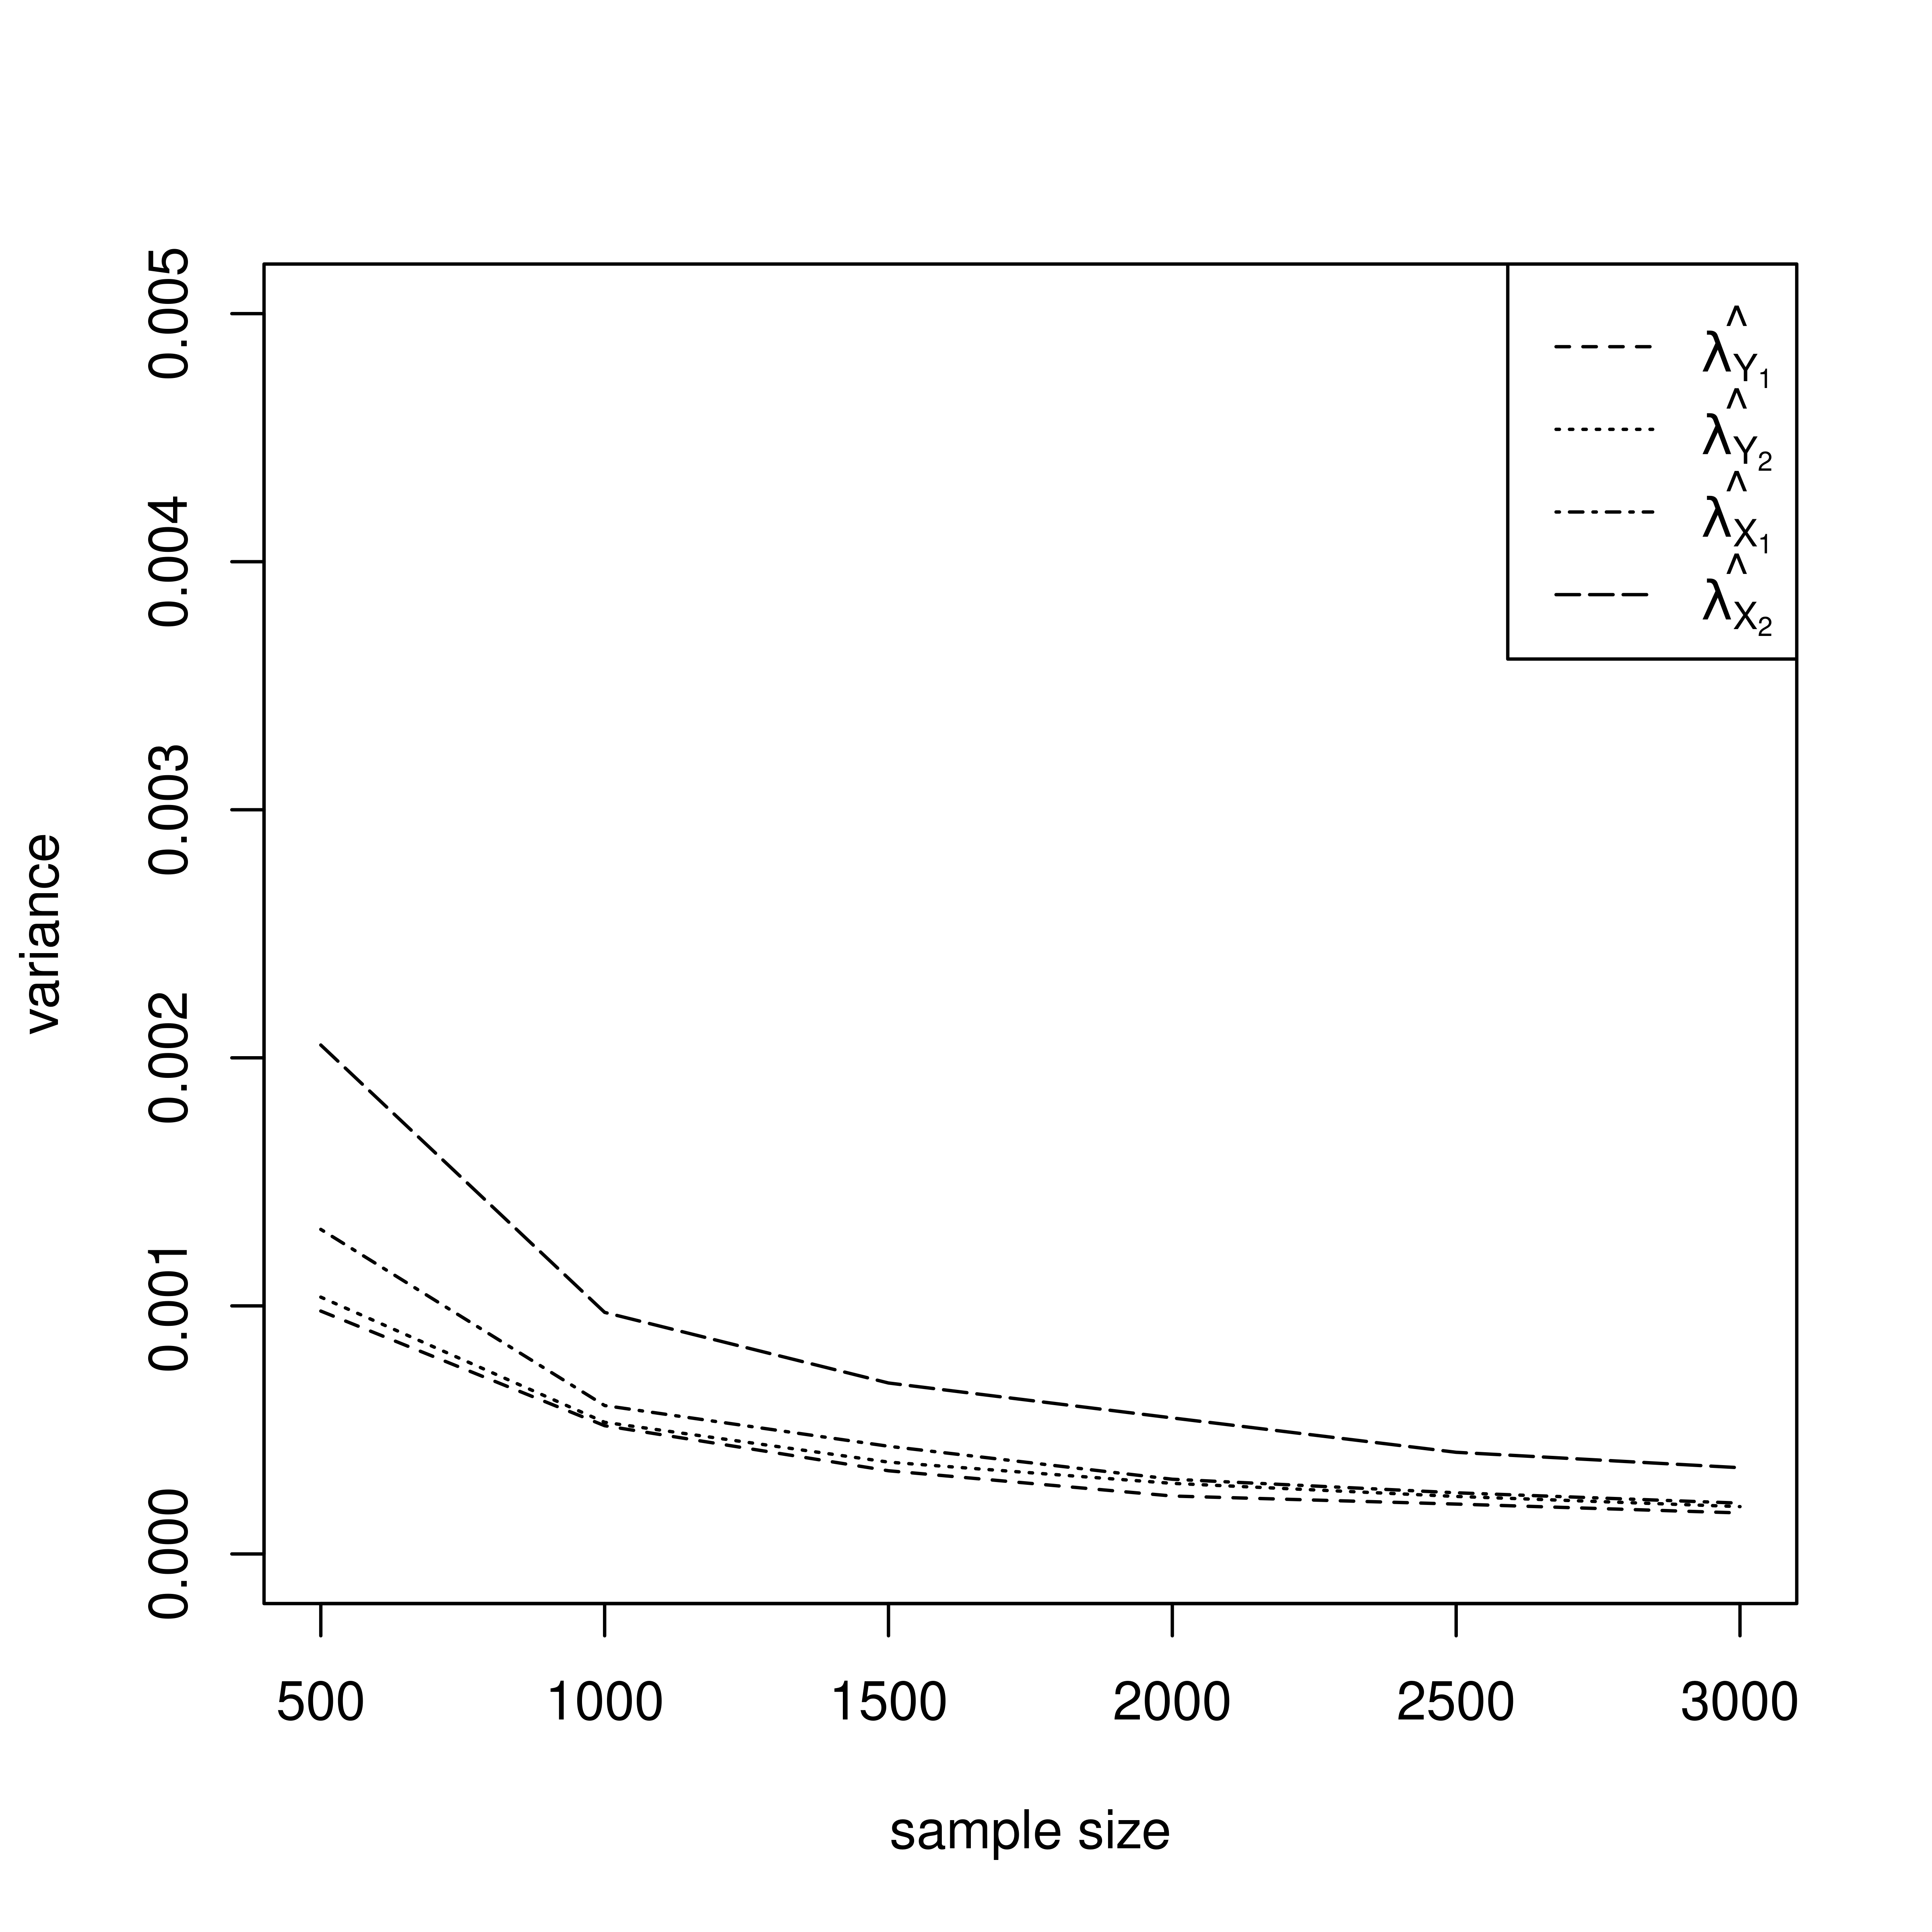
\includegraphics[width=\textwidth]{Fig/var_uneq_discrim_high.png}
	      \caption{Variance}
	    \end{subfigure}
	  \end{figure}
	\end{frame}

	\begin{frame}[t]\frametitle{A speech scoring example}
		\begin{itemize}
			\item The speaking section of an English language proficiency test.
			\item A listen-repeat task, The sentences vary in lengths and may situate
			in different scenarios such as presentations and campus tours.
			\item Each recorded response is scored by two different trained raters,
			scale from 0 to 5.
			\item The \textit{SpeechRater}\texttrademark of ETS provides features
			related to different dimensions of a speech. Composite scores on accuracy,
			pronunciation, fluency, and rhythm are computed.
			\item 7690 observations. Raters are randomly assigned.
		\end{itemize}
	\end{frame}

	\begin{frame}[t]\frametitle{Results: estimates}
		\begin{table}[!htbp]
	  \vspace*{2em}
	    \centering
	    \label{tab:coefs_real_data} 
	  \begin{tabular}{@{\extracolsep{5pt}} cccc} 
	  \\[-1.8ex]\hline 
	  \hline \\[-1.8ex] 
	   & CUBLP & BLP & $\hat{\blambda}$ \\ 
	  \hline \\[-1.8ex] 
	  rating 1 & $0.456$ & $0.433$ & $0.944$ \\ 
	  rating 2 & $0.452$ & $0.430$ & $0.944$ \\ 
	  accuracy & $0.144$ & $0.137$ & $0.839$ \\ 
	  pronunciation & $0.009$ & $0.009$ & $0.333$ \\ 
	  fluency & $0.017$ & $0.016$ & $0.400$ \\ 
	  rhythm & $0.025$ & $0.024$ & $0.468$ \\ 
	  \hline \\[-1.8ex] 
	  \end{tabular} 
	  \end{table}
	\end{frame}

	\begin{frame}[t]\frametitle{Results: BLP and CUBLP}
		\begin{figure}[t]
	    \centering
	    \begin{subfigure}[b]{0.45\textwidth}
	      \centering
	      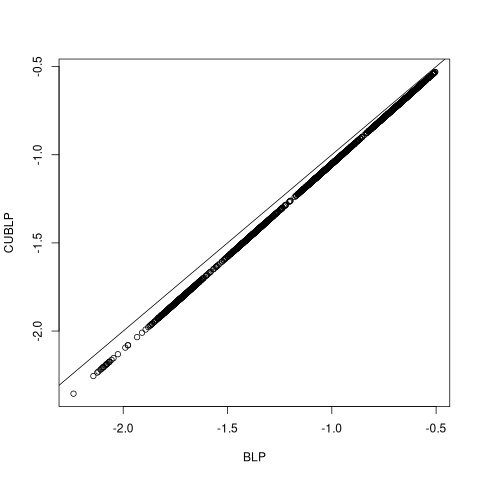
\includegraphics[width=\textwidth]{Fig/lower_S.png}
	      \caption{Lower performers}
	    \end{subfigure}
	    \begin{subfigure}[b]{0.45\textwidth}
	      \centering
	      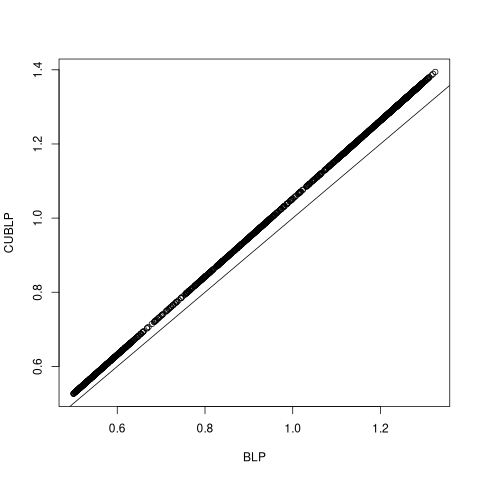
\includegraphics[width=\textwidth]{Fig/higher_S.png}
	      \caption{Higher performers}
	    \end{subfigure}
	  \end{figure}
	\end{frame}

	\begin{frame}[t]\frametitle{Discussion}
		\begin{itemize}
			\item Threats to fairness and equity.
			\item The algorithmic bias.
			\item The method is general and can be applied to a wide range of
			problems.
			\item Analyze a larger dataset.
		\end{itemize}
	\end{frame}

	\begin{frame}\frametitle{References}
		\printbibliography
	\end{frame}

	\begin{frame}[t]
		\begin{center}
		\vfill
	    \huge Thank you!\\
	    \huge xliu003@ets.org
	  \vfill
	  \end{center}
	\end{frame}
\end{document}